% !TEX program = pdflatex
% !TEX options = -synctex=1 -interaction=nonstopmode -file-line-error -shell-escape "%DOC%"
\documentclass{beamer}
\usepackage{graphicx,url}
\usepackage[brazil]{babel}   
\usepackage[utf8]{inputenc}
\usepackage{pgf,tikz}
\usepackage{adjustbox}
\usepackage{mathrsfs}
\usepackage{minted}
\usepackage{listings}
\usetikzlibrary{calc}
\usetikzlibrary{arrows}
\batchmode
\usepackage{amsmath,amssymb,enumerate,epsfig,bbm,calc,color,ifthen,capt-of}
\usetheme{Berlin}
%-------------------------Titulo/Autores/Orientador------------------------------------------------
\title[MCPC2020]{
  Monash Collegiate Programming Contest
}
\subtitle {Editorial}
\date{}
\author[Shizhe Zhao]{
  Shizhe Zhao
}

\pgfdeclareimage[height=0.7cm]{monash-logo}{icpc.pdf}
\logo{\pgfuseimage{monash-logo}\hspace*{0.5cm}}

\AtBeginSection[]
{
  \begin{frame}<beamer>
    \frametitle{Outline}
    \tableofcontents[currentsection]
  \end{frame}
}
\setbeamercovered{transparent}
% -----------------------------------------------------------------------------
\begin{document}
% -----------------------------------------------------------------------------

%---Summary---------------------------------------------------------
\frame{\titlepage}
\section[]{}
% \begin{frame}{Summary}
%   \tableofcontents
% \end{frame}

\begin{frame}{Cast}
  \begin{itemize}
    \item Coach: Shizhe Zhao
    \item Problem setters:
    \begin{itemize}
      \item Ali Toosi, Monash
      \item Jackson Goerner, Monash
      \item Shizhe Zhao, Monash
    \end{itemize}
    \item Tester: 
    \begin{itemize}
      \item Ali Khosravi, RMIT
      \item Sublimation, Xidian University
    \end{itemize}
  \end{itemize}
\end{frame}

\begin{frame}
  \frametitle{Storage Room I/II}
Author: Ali Toosi

\begin{itemize}
  \item Constraint: $1 \le V \le 10^3$
  \item Brute-force: try all possible $L, W, H$
  \item Common mistakes:
    \begin{itemize}
      \item float-point error
      \item incomplete search
      \item bad pruning (3 nested loops)
    \end{itemize}
\end{itemize}
\end{frame}


\begin{frame}
  \frametitle{Storage Room I/II}
Author: Ali Toosi

\begin{itemize}
  \item Constraint: $1 \le V \le 10^{12}$
  \item Observation: 
  \begin{itemize}
    \item assume $L \leq W \leq H$
    \item thus $L \leq W \leq \sqrt{V}$
    \item $L,W$ must be divisor of $V$
    \item \#divisors of $V$ in $[1, \sqrt{V}]$? Not too much!\footnote{\url{http://oeis.org/A066150}}
    \item Brute-force all possible $L, W$ in divisors.

  \end{itemize}
\end{itemize}
\end{frame}


\begin{frame}
  \frametitle{Fast and Furious I}
Author: Shizhe Zhao
\begin{itemize}
  \item Method 1: BFS - status \texttt{x, y, direction}.
  \item Method 2: Greedy - make $|dx - dy|$ as small as possible
\end{itemize}

\end{frame}

\begin{frame}
  \frametitle{Fast and Furious II}
Author: Shizhe Zhao
\begin{itemize}
  \item Dynamic programming: $dp(x,y,step,d)$
  \begin{itemize}
    \item $dp(x, y, step, d) \rightarrow dp(x', y', step+1, d')$
    \item $step \le 3 * (dx + dy) \approx 300$
    \item memory cost: $50 * 50 * 300 * 4 = 3 * 10^6$
  \end{itemize}
\end{itemize}

\end{frame}

\begin{frame}
  \frametitle{Hearty Frogger I/II}
Author: Jackson Goerner
\begin{figure}[]
  \centering
  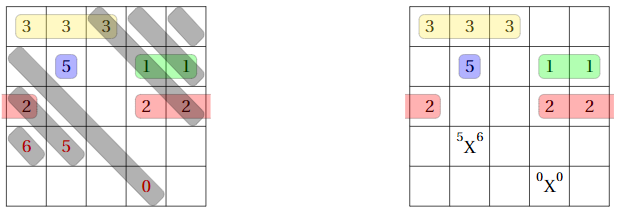
\includegraphics[width=.9\textwidth]{Diagonal.png}  
\end{figure}

\begin{itemize}
  \item Observation: change the frame of reference so that we can assume only Alice move,
  and she can take all hearts in left-up diagonal line.
  \item Thus, for version I, we can Brute-force all start and count values on left-up diagonal line.
\end{itemize}
\end{frame}

\begin{frame}
  \frametitle{Hearty Frogger I/II}
Author: Jackson Goerner
 \begin{figure}[]
  \centering
  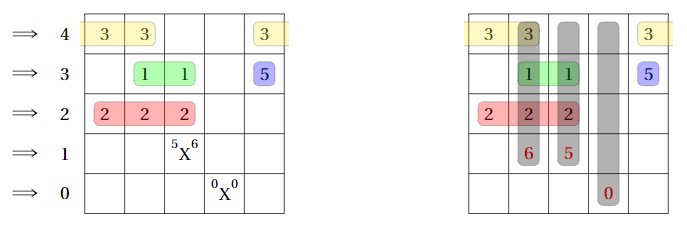
\includegraphics[width=.9\textwidth]{Shifting.png}  
\end{figure} 
\begin{itemize}
  \item \small For better visualization, we shift the $i$th row to right $b-i-1$ position.
  \item \small For a spawn location $(row, col, tl, tr)$, the best answer is $max(vert\_sum(i) | i \in [l', r'])$.
  \item \small This is a range query problem - assuming we already have the $vert\_sum$ from $0$ to $row$.
\end{itemize}
\end{frame}

\begin{frame}
  \frametitle{Hearty Frogger I/II}
Author: Jackson Goerner
 \begin{figure}[]
  \centering
  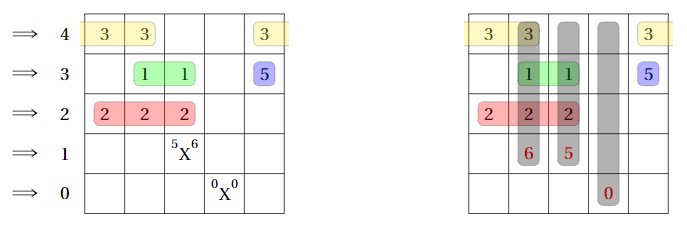
\includegraphics[width=.9\textwidth]{Shifting.png}  
\end{figure} 
\begin{itemize}
  \item \small We can maintain such array by: processing rows from top to bottom, adding trucks on each row -
  \item \small which is a range updating problem
  \item \small Both range query and range updating can be handled by segment tree.
\end{itemize}
\end{frame}

% -----------------------------------------------------------------------------
\end{document}
%-----------------------------------------------
